\documentclass[12pt]{article}
\usepackage[left=0.5in,top=0.5in,right=0.5in,bottom=0.5in,nohead]{geometry}
\usepackage{geometry}                % See geometry.pdf to learn the layout options. There are lots.
\geometry{a4paper}                   % ... or a4paper or a5paper or ... 
\usepackage{wrapfig}	%in-line figures
\usepackage{natbib}		%bibliography
\usepackage{pslatex} 	%for times new roman
\usepackage[parfill]{parskip}    % Activate to begin paragraphs with an empty line rather than an indent
\usepackage{graphicx}
\usepackage{amssymb}
\usepackage{epstopdf}
\usepackage{booktabs}
\usepackage{amsmath}
\usepackage{xfrac}
\usepackage{outlines}

\DeclareGraphicsRule{.tif}{png}{.png}{`convert #1 `dirname #1`/`basename #1 .tif`.png}

\author{Sean R. Hackett}
\title{Leveraging wide-data to improve protein quantification and inference} 
\date{}

\begin{document}

\setlength{\parskip}{1mm}
\linespread{1}

\thispagestyle{empty}
\pagestyle{empty}

\maketitle

\abstract{tmp}

\section{Background}

As biologists continue to search for a deeper understanding of their system, there is an increasing focus on analyzing the proteins and metabolites that are the primary effectors of physiology and metabolism. This increased interest has been enabled by improved analytical techniques for measuring these species, particularly liquid/gas chromatography (GC/LC) coupled mass spectrometry (MS). While the promise of mass spectrometry is great, the community is far from reaching a consensus on how mass spectrometry data should be best analyzed.

Most approaches either attempt to quantify peptides and then determine a protein-level consensus or attempt to simultaneously model protein and peptide abundances.


We determined that the primary statistical step should be in the analysis of peptides / metabolites. Previous approaches to quantify these species have noted that residuals are approximately log-normal with the presence of additional outliers, but 

, and then when a conversion from peptide to proteins is warranted 



rigorous treatment of the distribution of ion counts 



Rigorous analysis of mass spectrometry

Statistical methods for quantitative mass spectrometry proteomic experiments with labeling - Ann L Oberg* and Douglas W Mahoney - fit all proteins and peptides simultaneously and fit variance based on IC

peptide -> protein measurements assume independence of residuals

coupling protein-level inference

Here we propose an approach towards 

\begin{figure}
\begin{center}
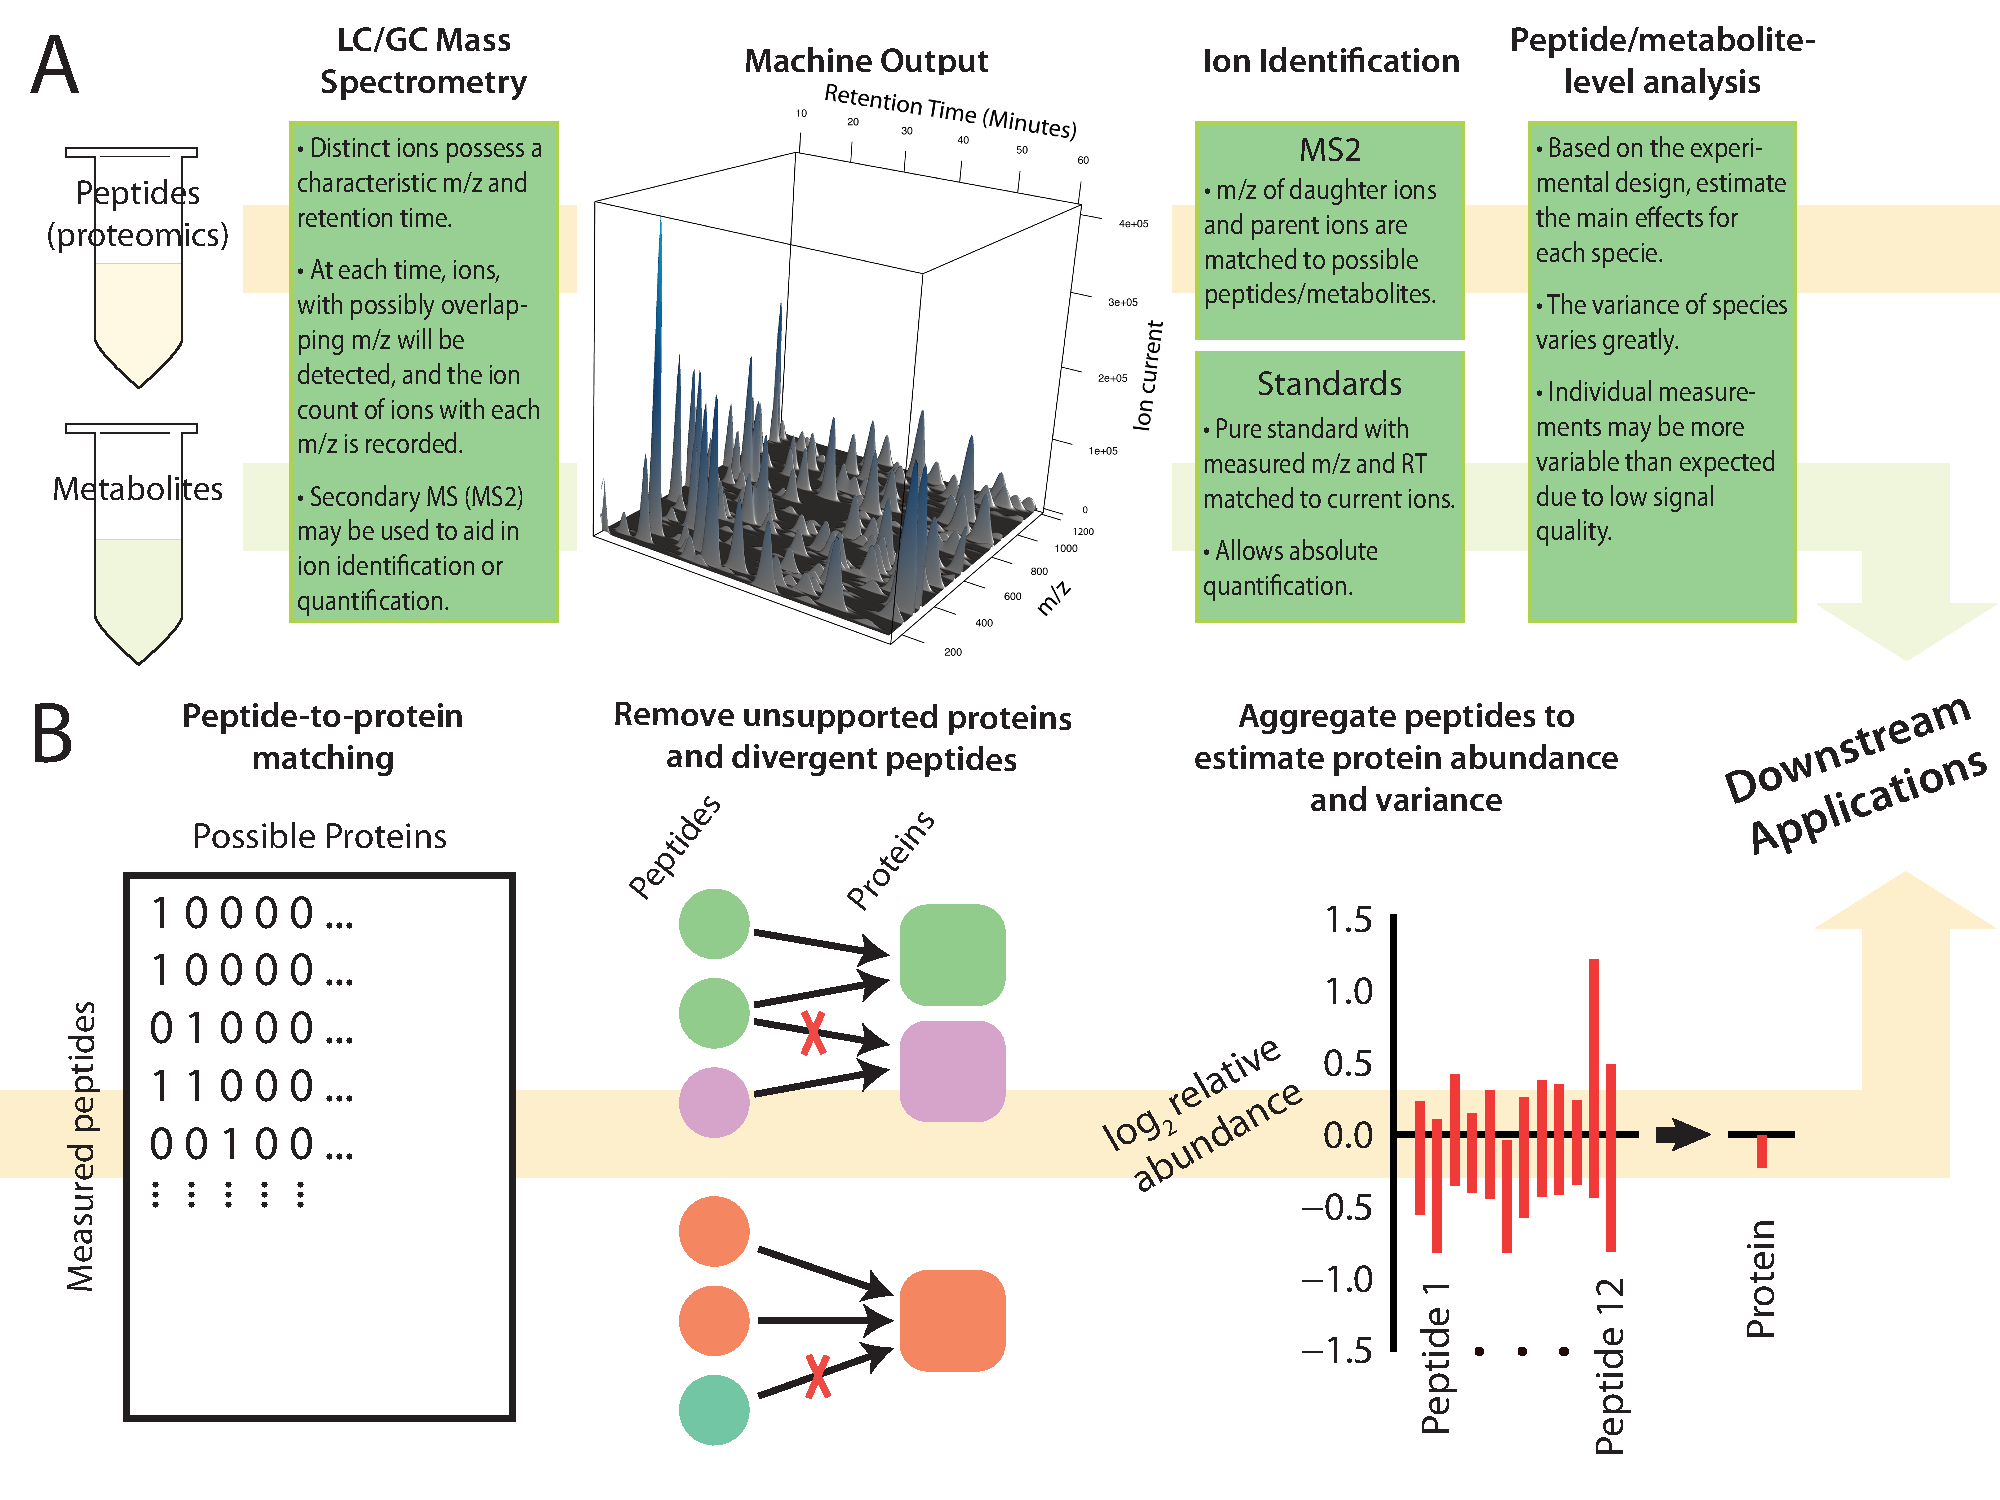
\includegraphics[width = 0.8\textwidth]{Figures/MSanalysis_agg.pdf}
\label{MSworkflow}
\caption{woot}
\end{center}
\end{figure}

\section{Results}

Consider the inference of peptide abundances in two proteomics datasets and the inference of metabolite abundance in a metabolomics dataset

\subsection{Investigating sources of variation in mass spectrometry data}

Whether determining the concentration of metabolites during metabolomics, or peptides during proteomics, a quantitative mass spectrometry experiment generally entails determining the relative abundances of ions across a set of samples.  As the abundances of ions will be correlated with the total sample concentration, the concentration of samples should be proportional to the \textit{in vivo} concentration of peptides/metabolites.  In general, \textit{in vivo} concentrations will not vary greatly, except perhaps when comparing the composition of different tissues, so differences in overall signal are generally best dealt with by preparing samples of equal concentration. To further minimize the systematic error from differences in sample concentration, each sample can be normalized relative to an ``average sample'' using an approach such as the robust median polish (Equation \textcolor{red}{eq}). 

plot(peptide sd versus IC)


In order use mass spectrometry data to appropriately estimate the value of design covariates, and their uncertainty, an appropriate statistical relationship between ion counts and the experimental design must be formed. As a preliminary assessment of which class(es) of regression models may be most appropriate for mass spectrometry data, three alternative parametric parametric models of ion-count abundance were tested: treating ion counts as normally distributed, log-normally distributed or treating ion counts as count data following a negative binomial distribution.



From this investigation it is clear that a log-normal model of ion abundance conforms far better to the data than a normal model or negative binomial model. The superiority of the log-normal model is because for a given peptide there is a nearly constant multiplicative error, although this relative error clearly does decrease when comparing ions with very high-signal to those with very low-signal.  While the log-normal distribution is the only tested model which can model this type of error variance, which is regularly amenable to regression, this does not require that the log-normal distribution is a good model of ion abundance.  Other distributions might be a more appropriate model of ion count abundance, but the ready application to regression and well understood properties of the normal distribution, make its use highly valuable if its use it appropriate.





Differences between log-normal and frichet


For each of \textcolor{red}{x} peptides considered, the three alternative models were fitte

 across the samples while correcting for ,


ion counts of different mass spectrometry experiments must be compared.  

Determining the relationship between teh 



\subsubsection{Homoschedastic models}

As a preliminary assessment of which class(es) of regression models may be most appropriate for mass spectrometry data, 

Using the large proteomic dataset of Foss et al. 2007 we investigated what an appropriate model of ion count abundance across the 

,d 

\textcolor{red}{fixed effects models for each data set}

\subsubsection{Evaluating the appropriateness of a log-normal model of mass spectrometry data}




\end{document}